\documentclass[a4paper,12pt]{article}

%%% Работа с русским языком
\usepackage{cmap}					% поиск в PDF
\usepackage{mathtext} 				% русские буквы в формулах
\usepackage[T2A]{fontenc}			% кодировка
\usepackage[utf8]{inputenc}			% кодировка исходного текста
\usepackage[english,russian]{babel}	% локализация и переносы

%%% Дополнительная работа с математикой
\usepackage{amsmath,amsfonts,amssymb,amsthm,mathtools} % AMS
\usepackage{icomma} % "Умная" запятая: $0,2$ --- число, $0, 2$ --- перечисление

%% Номера формул
%\mathtoolsset{showonlyrefs=true} % Показывать номера только у тех формул, на которые есть \eqref{} в тексте.
%\usepackage{leqno} % Нумерация формул слева

%% Свои команды
\DeclareMathOperator{\sgn}{\mathop{sgn}}

%% Перенос знаков в формулах (по Львовскому)
\newcommand*{\hm}[1]{#1\nobreak\discretionary{}
{\hbox{$\mathsurround=0pt #1$}}{}}

%%% Работа с картинками
\usepackage{graphicx}  % Для вставки рисунков
\graphicspath{{materials}{images2/}}  % папки с картинками
\setlength\fboxsep{3pt} % Отступ рамки \fbox{} от рисунка
\setlength\fboxrule{1pt} % Толщина линий рамки \fbox{}
\usepackage{wrapfig} % Обтекание рисунков текстом

%%% Работа с таблицами
\usepackage{array,tabularx,tabulary,booktabs} % Дополнительная работа с таблицами
\usepackage{longtable}  % Длинные таблицы
\usepackage{multirow} % Слияние строк в таблице

%%% Теоремы
\theoremstyle{plain} % Это стиль по умолчанию, его можно не переопределять.
\newtheorem{theorem}{Теорема}[section]
\newtheorem{proposition}[theorem]{Утверждение}
 
\theoremstyle{definition} % "Определение"
\newtheorem{corollary}{Следствие}[theorem]
\newtheorem{problem}{Задача}[section]
 
\theoremstyle{remark} % "Примечание"
\newtheorem*{nonum}{Решение}

%%% Программирование
\usepackage{etoolbox} % логические операторы

%%% Страница
%\usepackage{extsizes} % Возможность сделать 14-й шрифт
\usepackage{geometry} % Простой способ задавать поля
	\geometry{top=25mm}
	\geometry{bottom=30mm}
	\geometry{left=25mm}
	\geometry{right=25mm}
 %

%%% Способ сделать тоже самое(но красивее:)
%\usepackage[margin=0.8in]{geometry}

 
\usepackage{fancyhdr} % Колонтитулы
 	\pagestyle{fancy}
 	\renewcommand{\headrulewidth}{0mm}  % Толщина линейки, отчеркивающей верхний колонтитул
 	\lfoot{}
 	\rfoot{}
 	\rhead{}
 	\chead{}
 	\lhead{ }
 	% \cfoot{Нижний в центре} % По умолчанию здесь номер страницы

\usepackage{setspace} % Интерлиньяж
%\onehalfspacing % Интерлиньяж 1.5
%\doublespacing % Интерлиньяж 2
%\singlespacing % Интерлиньяж 1

\usepackage{lastpage} % Узнать, сколько всего страниц в документе.

\usepackage{soulutf8} % Модификаторы начертания

\usepackage{hyperref}
\usepackage[usenames,dvipsnames,svgnames,table,rgb]{xcolor}
\hypersetup{				% Гиперссылки
    unicode=true,           % русские буквы в раздела PDF
    pdftitle={Заголовок},   % Заголовок
    pdfauthor={Автор},      % Автор
    pdfsubject={Тема},      % Тема
    pdfcreator={Создатель}, % Создатель
    pdfproducer={Производитель}, % Производитель
    pdfkeywords={keyword1} {key2} {key3}, % Ключевые слова
    colorlinks=true,       	% false: ссылки в рамках; true: цветные ссылки
    linkcolor=red,          % внутренние ссылки
    citecolor=green,        % на библиографию
    filecolor=magenta,      % на файлы
    urlcolor=blue           % на URL
}

%\renewcommand{\familydefault}{\sfdefault} % Начертание шрифта

\usepackage{multicol} % Несколько колонок

% Мои "дополнительные" пакеты
\usepackage{textcase} 
\usepackage{pdfpages}
\usepackage{amsmath}
\usepackage{titlesec}
\usepackage{floatrow}

\usepackage[table,xcdraw]{xcolor} %цветная табличка

\author{Подкидышев Алексей}
\title{Студент МФТИ ФИВТ - 1ый курс}
\date{\today}

%% Делаем красивый header:
\fancyhead[RO]{\footnotesize{\scshape\nouppercase{~\leftmark}}}
%% Делаем красивый header END

%Делаем большой отступ между section и subsection
\titlespacing*{\section} {0pt}{3.5ex plus 1ex minus .2ex}{2.7ex plus .2ex}
\titlespacing*{\subsection} {0pt}{2.7ex plus 1ex minus .2ex}{1ex plus .2ex}


\begin{document} % конец преамбулы, начало документа

\begin{center}
	\textit{\MakeTextUppercase{федеральное государственное автономное учреждение}}
		
	\vspace{0.5ex}
	
	\textbf{ \\ \MakeTextUppercase{<<Московский Физико-технический институт>>}}
\end{center}
\vspace{13ex}
\begin{flushright}
	\noindent
	{
	Подкидышев Алексей Сергеевич}
	\\
	\textit{Студенты факультета инноваций\\ и высоких технологий\\(группа 792)}
\end{flushright}
\begin{center}
	\vspace{23ex}
	\line(1,0){430}\\[4ex]
	{\LARGE\textbf{Лабораторная работа 8.1}}
	\vspace{2ex}\\
	\textbf{\large{<<Определение постоянных Стефана-Больцмана и Планка из анализа теплового излучения накаленного тела>>}}\\[3ex]
	\line(1,0){430}\\[5ex]
	\vfill
	Долгопрудный 
	
	{\today}
\end{center}

\newpage
\newpage
\renewcommand{\headrulewidth}{1pt}

\section{Описание работы}

\subsection{Экспериментальная установка}

\begin{figure}[h]
        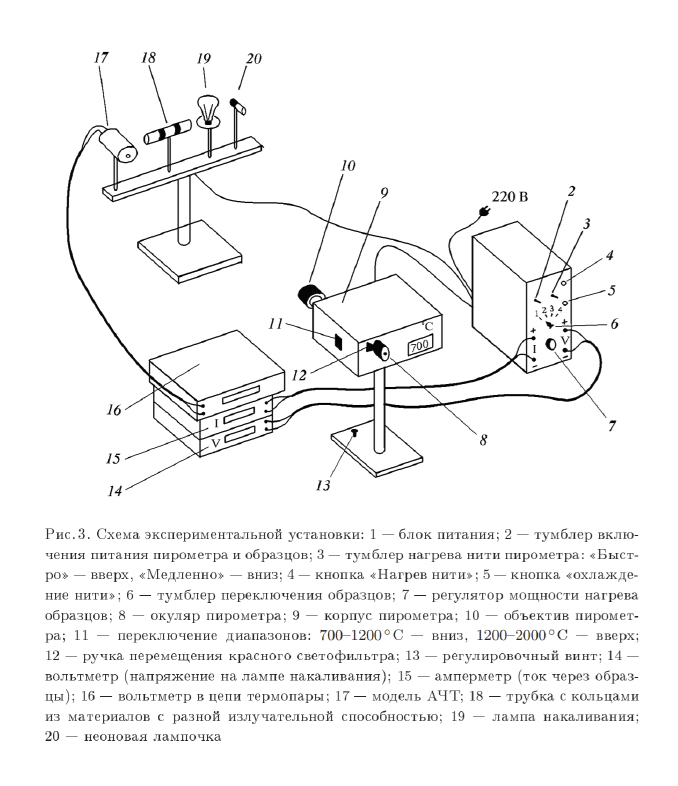
\includegraphics[width=0.7 \textwidth]{Materials/scheme.jpg}
    \caption{Схема установки}
\end{figure}

\subsection{ТеорЕтическая часть}
\indent Различают три температуры, функционально связанные с истинной термодинамической температурой и излучательной способностью тела: радиационную $T_\text{рад}$, цветовую $T_\text{цвет}$, и яркостную
$T_\text{ярк}$.\\
\indent Под радиационной температурой понимают температуру АЧТ, при которой его интегральная испускательная способность одинакова с интегральной испускательной способностью исследуемого тела.
Под цветовой температурой исследуемого тела понимают температуру АЧТ, при которой отношение их спектральных испускательных способностей для двух заданных длин волн одинаково.\\
\indent Под яркостной температурой понимают температуру АЧТ, при которой его спектральная испускательная способность равна спектральной испускательной способности исследуемого тела при той же длине волны. Её мы и будем измерять. \\
\indent Если бы нить излучала как АЧТ, то баланс потребляемой и излучаемой энергии определялся бы соотношением:
\begin{equation}
    W = \sigma S (T^4 - T_0^4)
\end{equation}
\indent Излучение серого тела ослаблено по сравнению с излучением черного тела в $\epsilon T$ раз для любой длины волны при данной температуре $T$.\\
\indent Если предположить, что нить излучает как серое тело, то выражение (1) можно записать в виде:
\begin{equation}
    W = \varepsilon_T \sigma S T^4
\end{equation}

Из формулы (2) можно определить величину постоянной $\sigma$ в законе Стефана-Больцмана.

\section{Ход Работы}
\begin{enumerate}
    \item Значение термопары 41 $\dfrac{\text{мкв}}{{C}}$
    \item Значение $T_\text{ярк}$ АЧТ, измеренное при помощи пирометра — 1069 $C$ значение $T_\text{ярк}$ АЧТ, измеренное при помощи термопары — $1094$.
    \item Измерили $T_\text{ярк}$ для поверхности керамической трубы — 741 $C$; правого кольца — 708 $C$; левого кольца — 700 $C$.
    \item Постепенно увеличивая накал нити через каждые 100C, будем измерять $T_\text{ярк}$, а также будем записывать значения силы тока и напряжения, чтобы вычислить мощность, потребляемую нитью лампы.
    \item 
    Результаты представим в виде графиков $W =f1(T)$ $ln W =ln \varepsilon_T B + n lnT$,т.е. $lnW = f2(lnT)$. Величину $n$ определим как тангенс угла наклона в области высоких температур. Значение $\varepsilon T$ для вольфрама — 0,31. Вычисляем тангенс угла наклона в области высоких температур: $n = 3.941$, что довольно близко к 4.

% Please add the following required packages to your document preamble:
% \usepackage[table,xcdraw]{xcolor}
% If you use beamer only pass "xcolor=table" option, i.e. \documentclass[xcolor=table]{beamer}
\begin{table}[]
\begin{tabular}{|l|l|l|l|}
\hline
\rowcolor[HTML]{FFCC67} 
{\color[HTML]{000000} T, grad} & {\color[HTML]{000000} V} & {\color[HTML]{000000} W} & I     \\ \hline
909                            & 26,94                    & 21,47118                 & 0,797 \\ \hline
1010                           & 36,21                    & 33,05973                 & 0,913 \\ \hline
1115                           & 42,39                    & 41,71176                 & 0,984 \\ \hline
1208                           & 50,51                    & 54,29825                 & 1,075 \\ \hline
1310                           & 61,08                    & 72,19656                 & 1,182 \\ \hline
1413                           & 70,65                    & 90,22005                 & 1,277 \\ \hline
1556                           & 86,32                    & 122,747                  & 1,422 \\ \hline
1608                           & 98,66                    & 150,3578                 & 1,524 \\ \hline
1729                           & 107,91                   & 172,8718                 & 1,602 \\ \hline
1837                           & 119,11                   & 201,2959                 & 1,69  \\ \hline
1912                           & 132,04                   & 235,6914                 & 1,785 \\ \hline
\end{tabular}
\end{table}

\item Для каждого измеренного $T$ вычислим постоянную Стефана-Больцмана пр формуле: 
$\sigma = \dfrac{W}{\varepsilon_T S T^4}$ где $S = 0.36 \text{cm}^2$ а также постоянную Планка по формуле: 
\[ h = \sqrt[3]{\dfrac{2 \pi^5 k_B^4}{15 \sigma c^2}} \]

\end{enumerate}

\begin{figure}[H]
        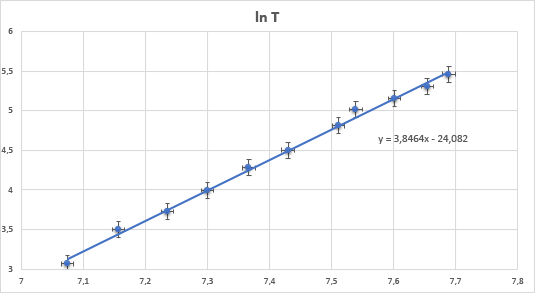
\includegraphics[width=0.89 \textwidth]{Materials/graph.png}
    \caption{График зависимости $ln W$ от $ln T$. В качаесте линии тренда используется метод наименьших квадратов, встроенный в MS Excel }
\end{figure}


\newpage
\subsection{Подсчет погрешностей}

\begin{minipage}{0.4\textwidth}
Так как 
\[\sigma = \dfrac{W}{\varepsilon_T S T^4},\]
то 
\[\varepsilon_\sigma = \varepsilon_W + \varepsilon_{\varepsilon_T} + \varepsilon_S + \varepsilon_{T^4},\]
где $\varepsilon_T = const, S = const,$ значит $\varepsilon_{\varepsilon_T} = 0, \varepsilon_S = 0.$
Так как $W = IU,$ то $\varepsilon_W = \varepsilon_I + \varepsilon_U.$ Учтем, что $\varepsilon_{T^4} = 4\varepsilon_T.$
\[\varepsilon_\sigma = \varepsilon_I + \varepsilon_U + 4\varepsilon_T.\]
При этом 
\[\varepsilon_h = \frac{1}{3}\cdot \varepsilon_\sigma.\]
\end{minipage}
\hfill
\begin{minipage}{0.45\textwidth}

Погрешности приборов:
\[\Delta U = 0,01 \textbf{В}, \Delta I = 0,01 \textbf{А}.\]
Из серии измерений для АЧТ возьмем погрешность пирометра:
\[\Delta T = 32 K.\]
Тогда имеем, что для $T = $
\[\varepsilon_\sigma = \frac{\Delta I}{I} + \frac{\Delta U}{U} + 4\cdot\frac{\Delta T}{T} \]
\[\varepsilon_h = \frac{1}{3}\varepsilon_\sigma .\]
\end{minipage}

Таким образом
\[\Delta \sigma = \varepsilon_\sigma \cdot \sigma = 0.32\]
\[\Delta h = \varepsilon_h \cdot h = 0.11 .\]
\section{Вывод}
При помощи АЧТ провели измернеия температуры оптическим пирометром с исчезающей нитью и термопарой. Мы ознакомились с теорией излучения АЧТ, получили значения постоянных Стефана-Больцмана и Планка, которые хорошо соответсвутют табличным значениям:\\
\[ \sigma = (5.46 \pm 0.32) \cdot 10^{-8} \text{Вт м К}, \] 
\[ h = (6.69 \pm 0.11) 10 ^{-34} \text{Дж с} \]

\newpage

\section{Отзывы}

\begin{center}
    \textbf{См на пометки ручки}
\end{center}


\begin{figure}[h]
        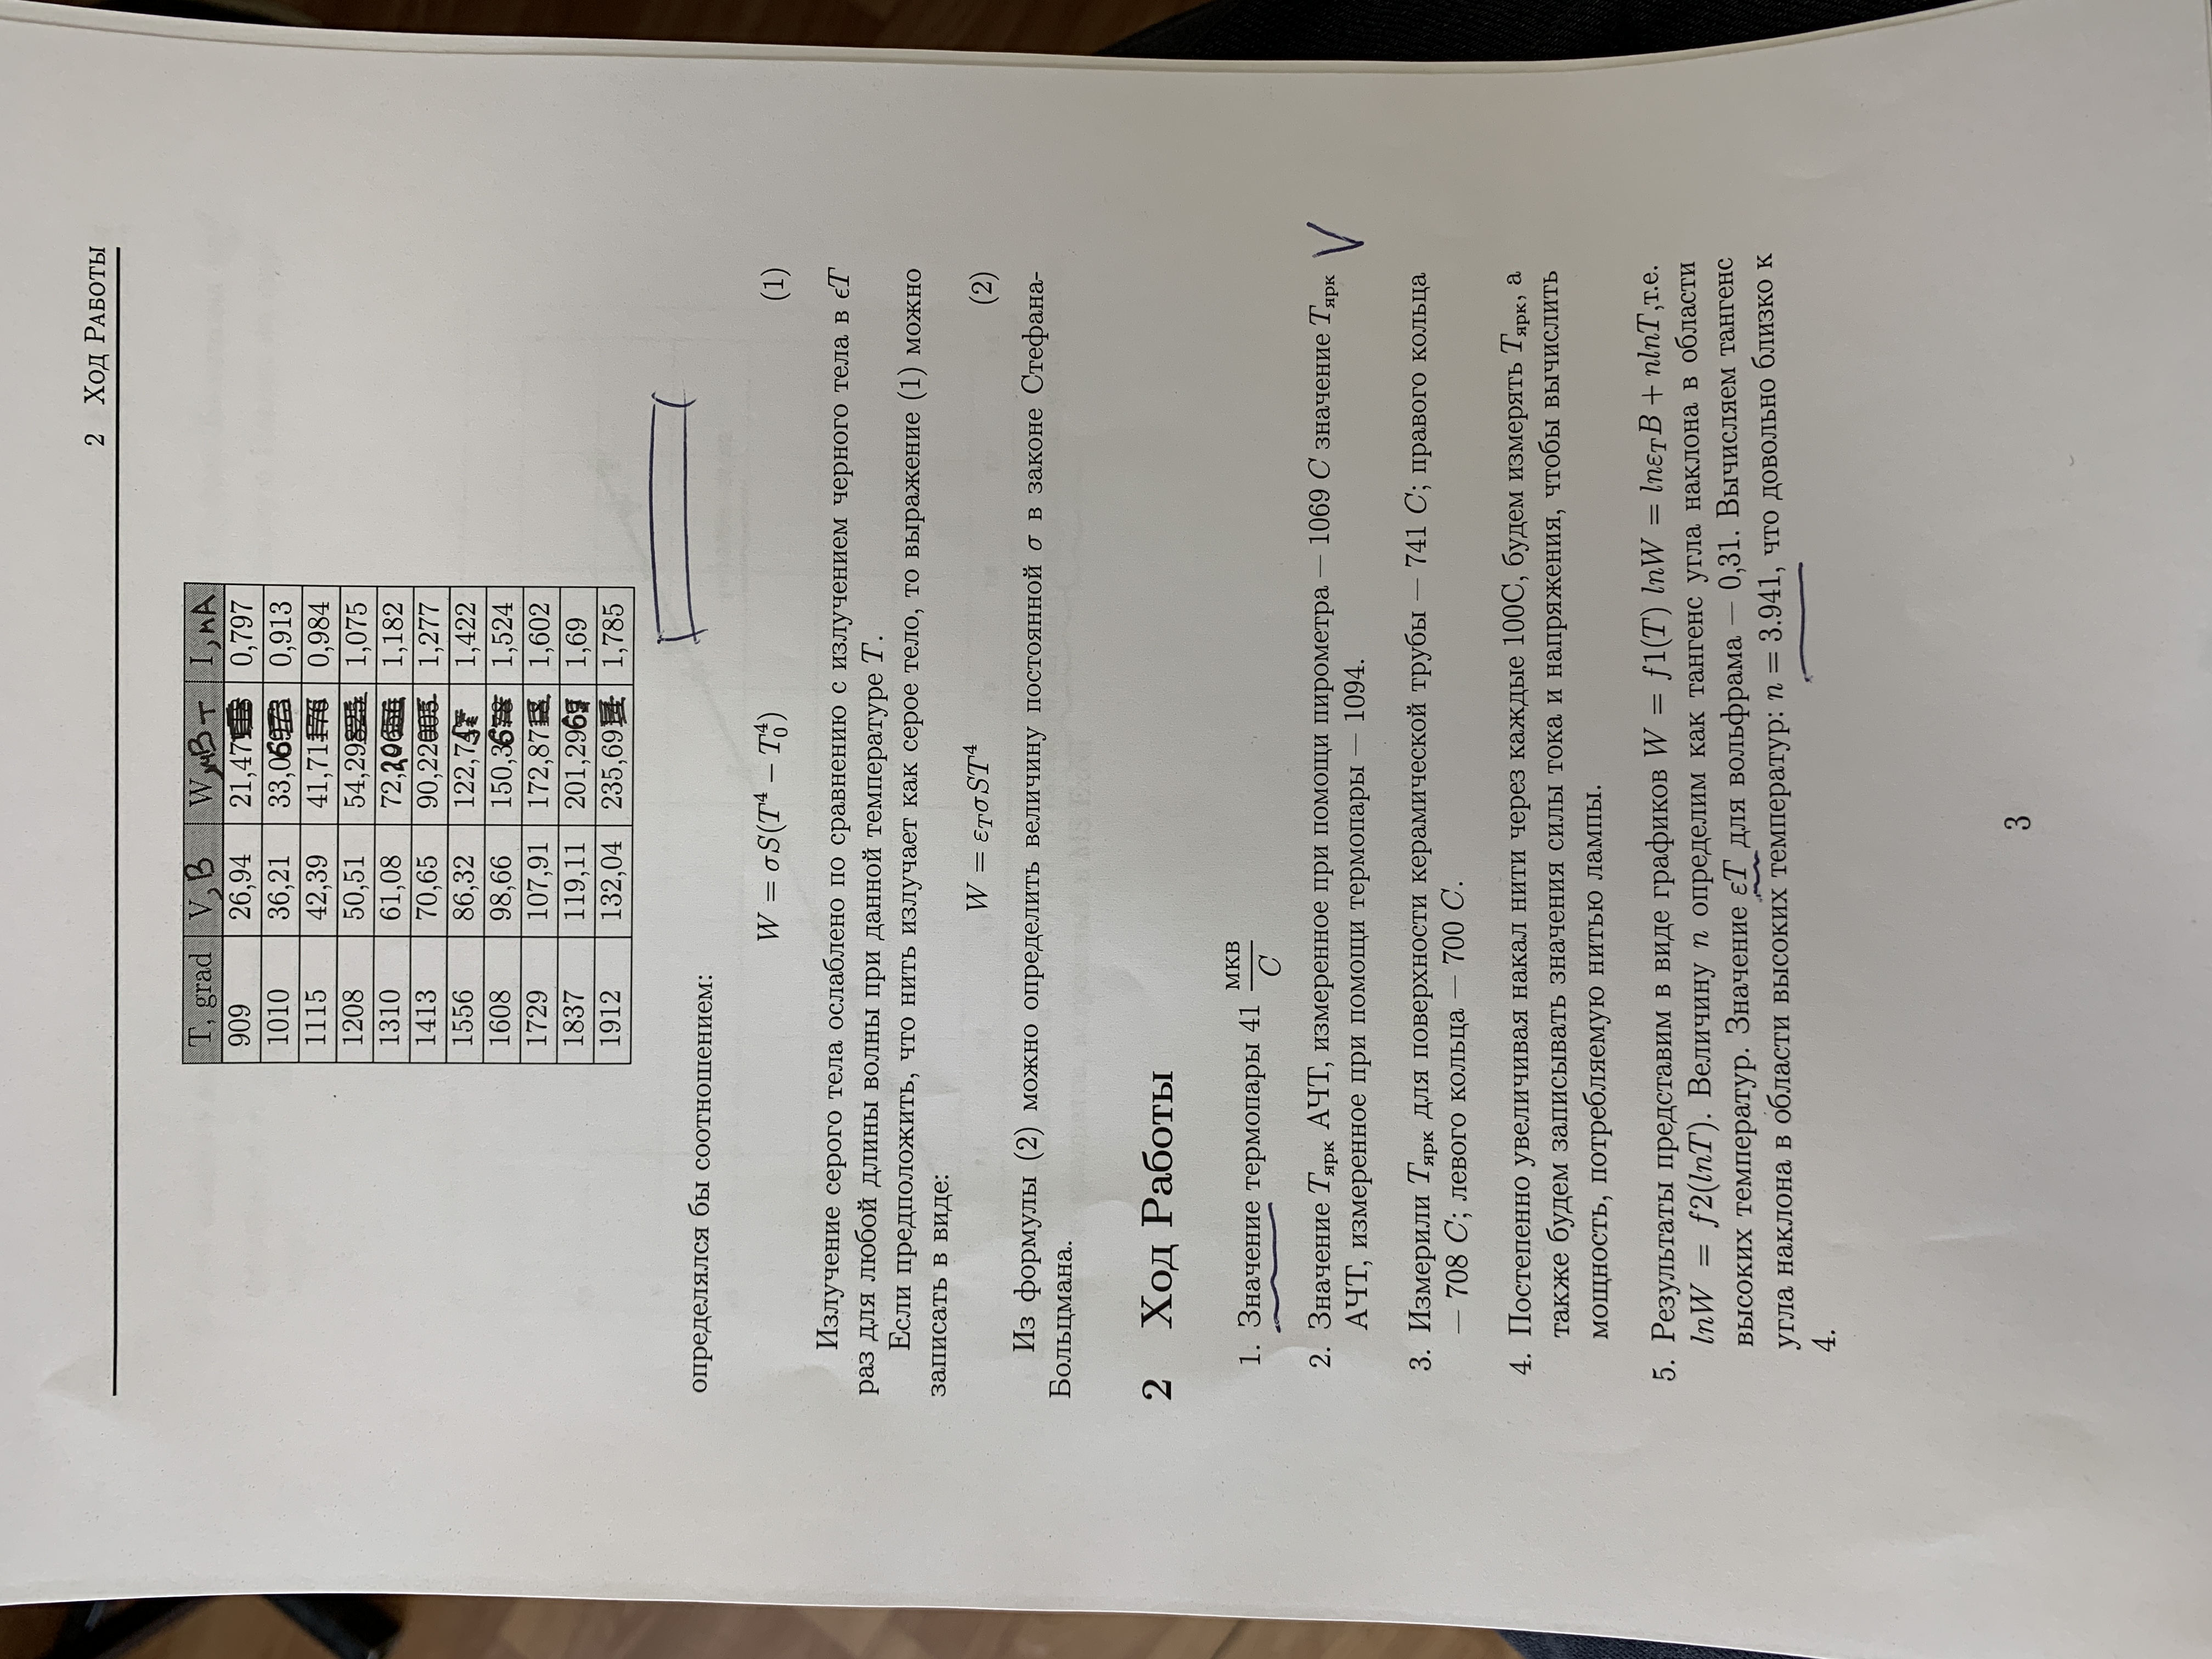
\includegraphics[width=1 \textwidth, angle = 270]{Materials/graph/IMG_2481.JPG}
    \caption{Схема установки}
\end{figure}


\begin{figure}[h]
        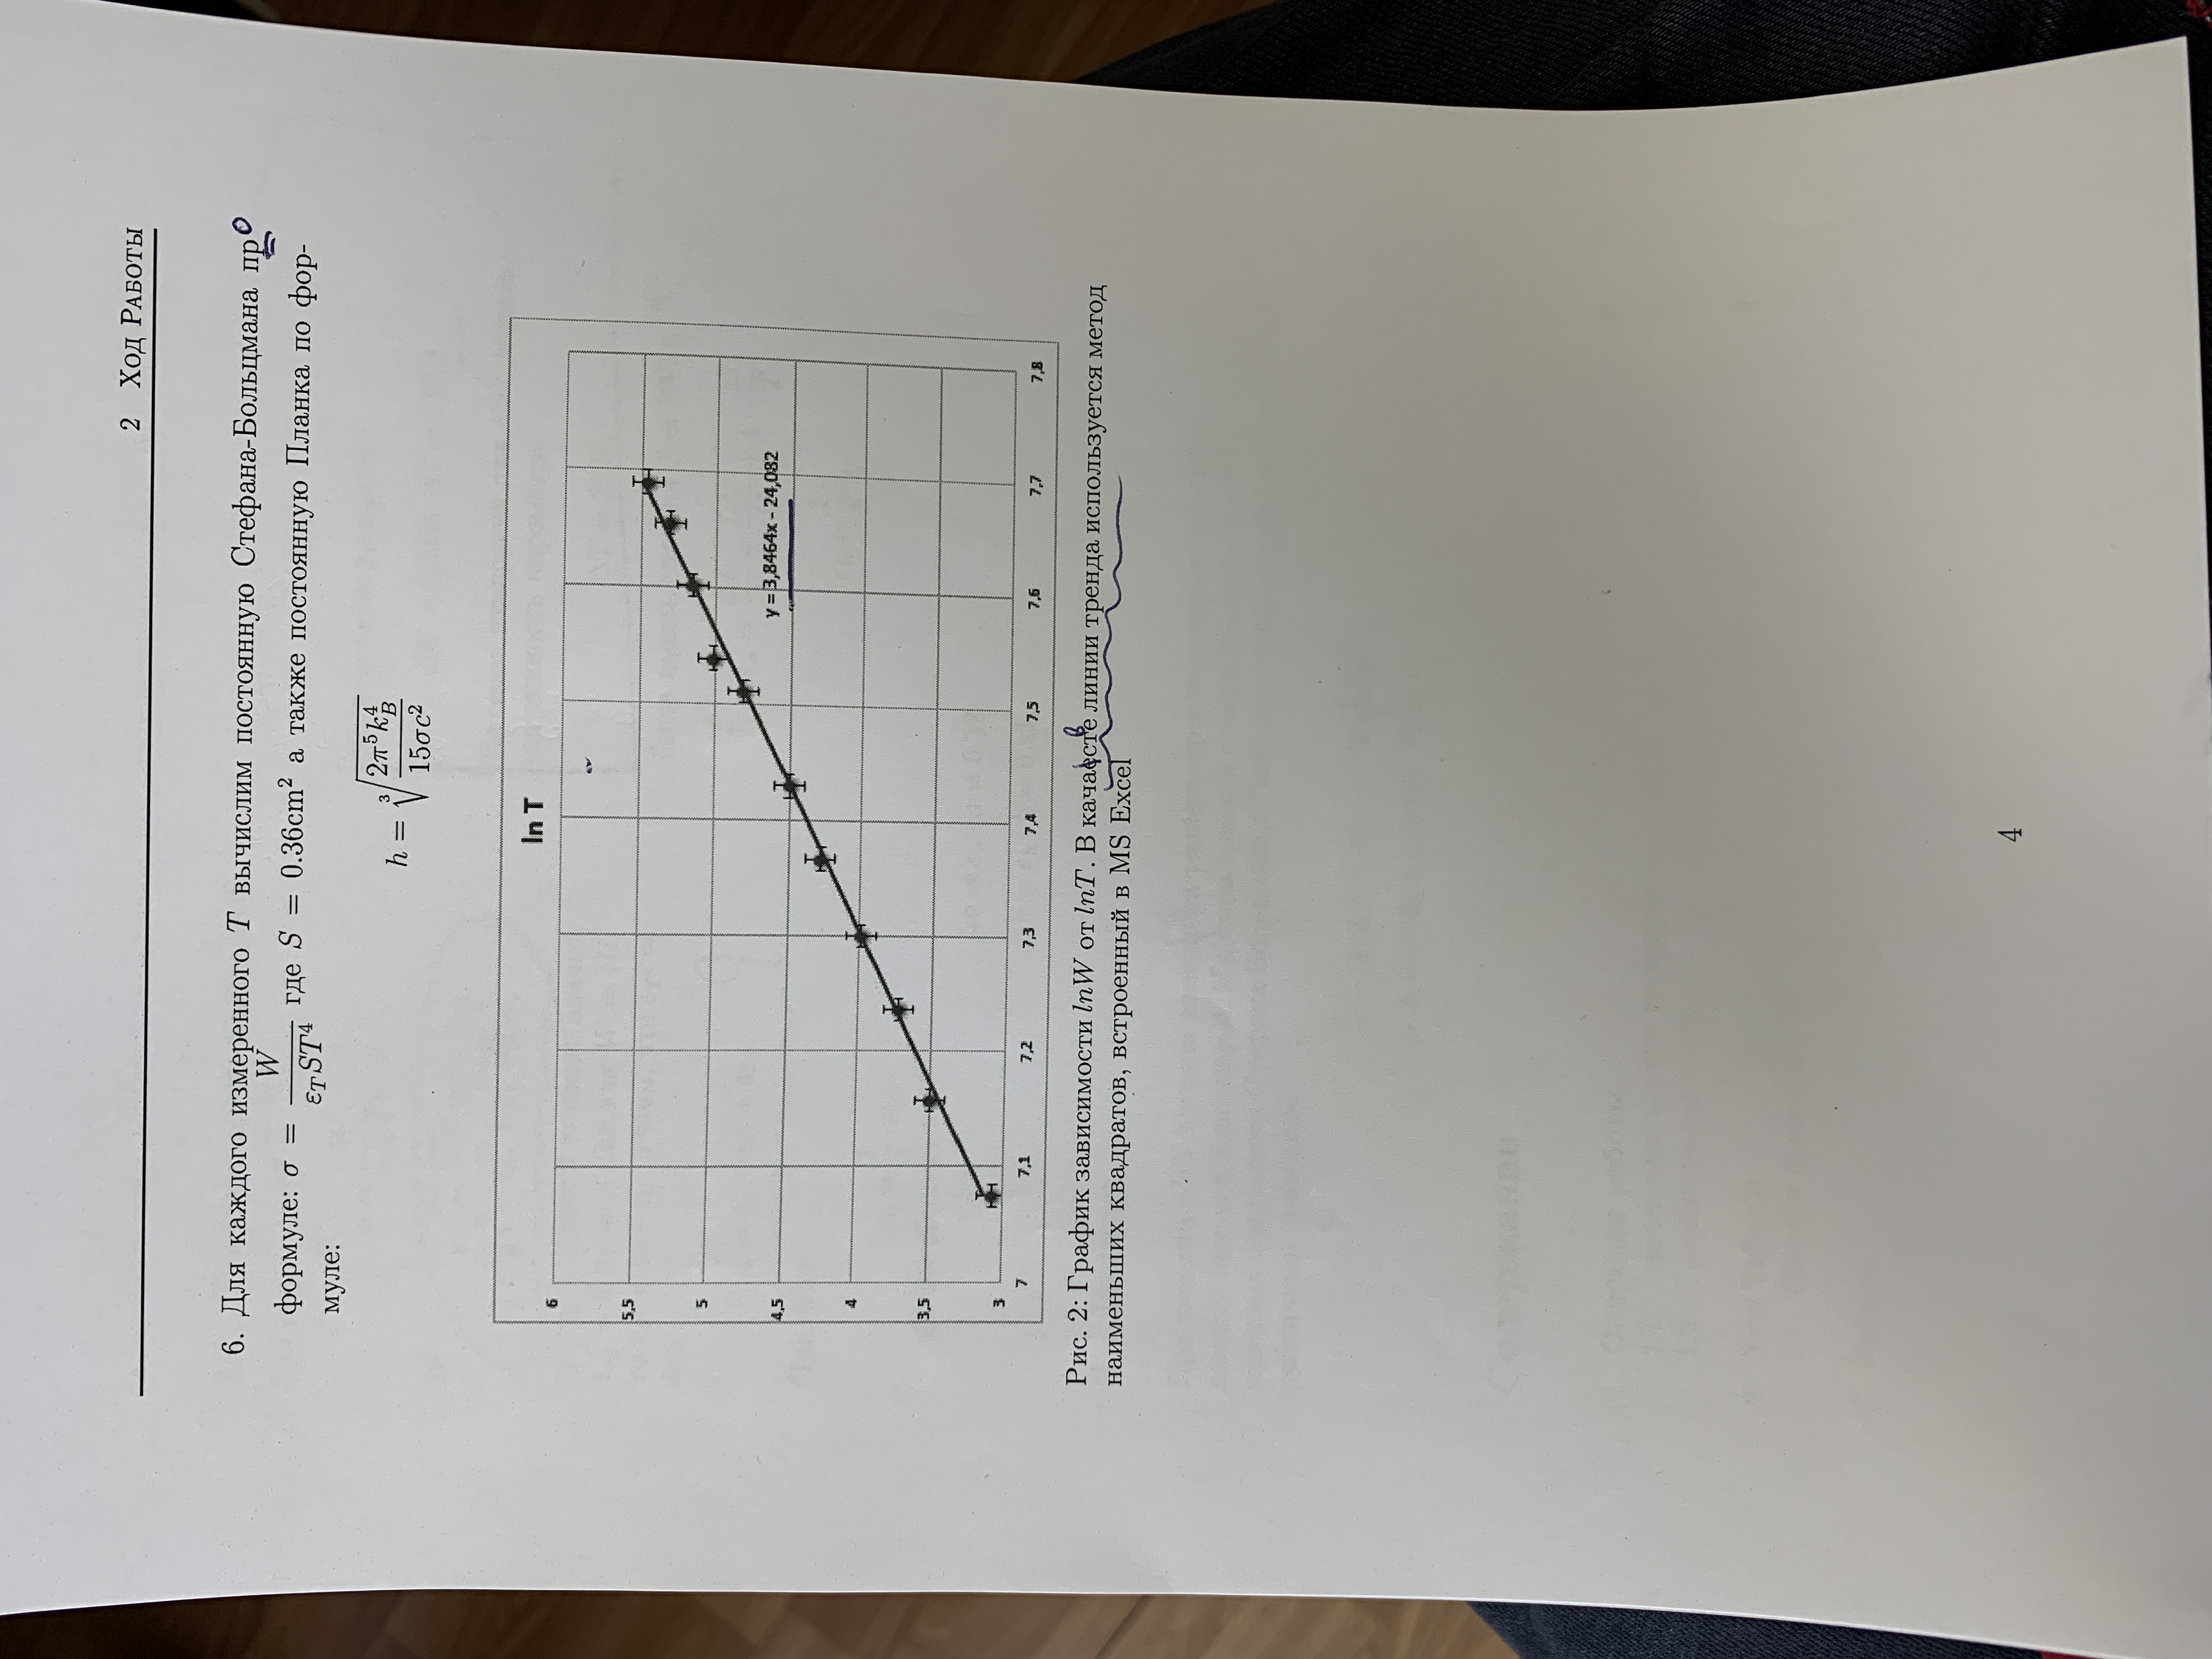
\includegraphics[width=1 \textwidth,angle = 270]{Materials/graph/IMG_2482.JPG}
    \caption{Схема установки}
\end{figure}


\begin{figure}[h]
        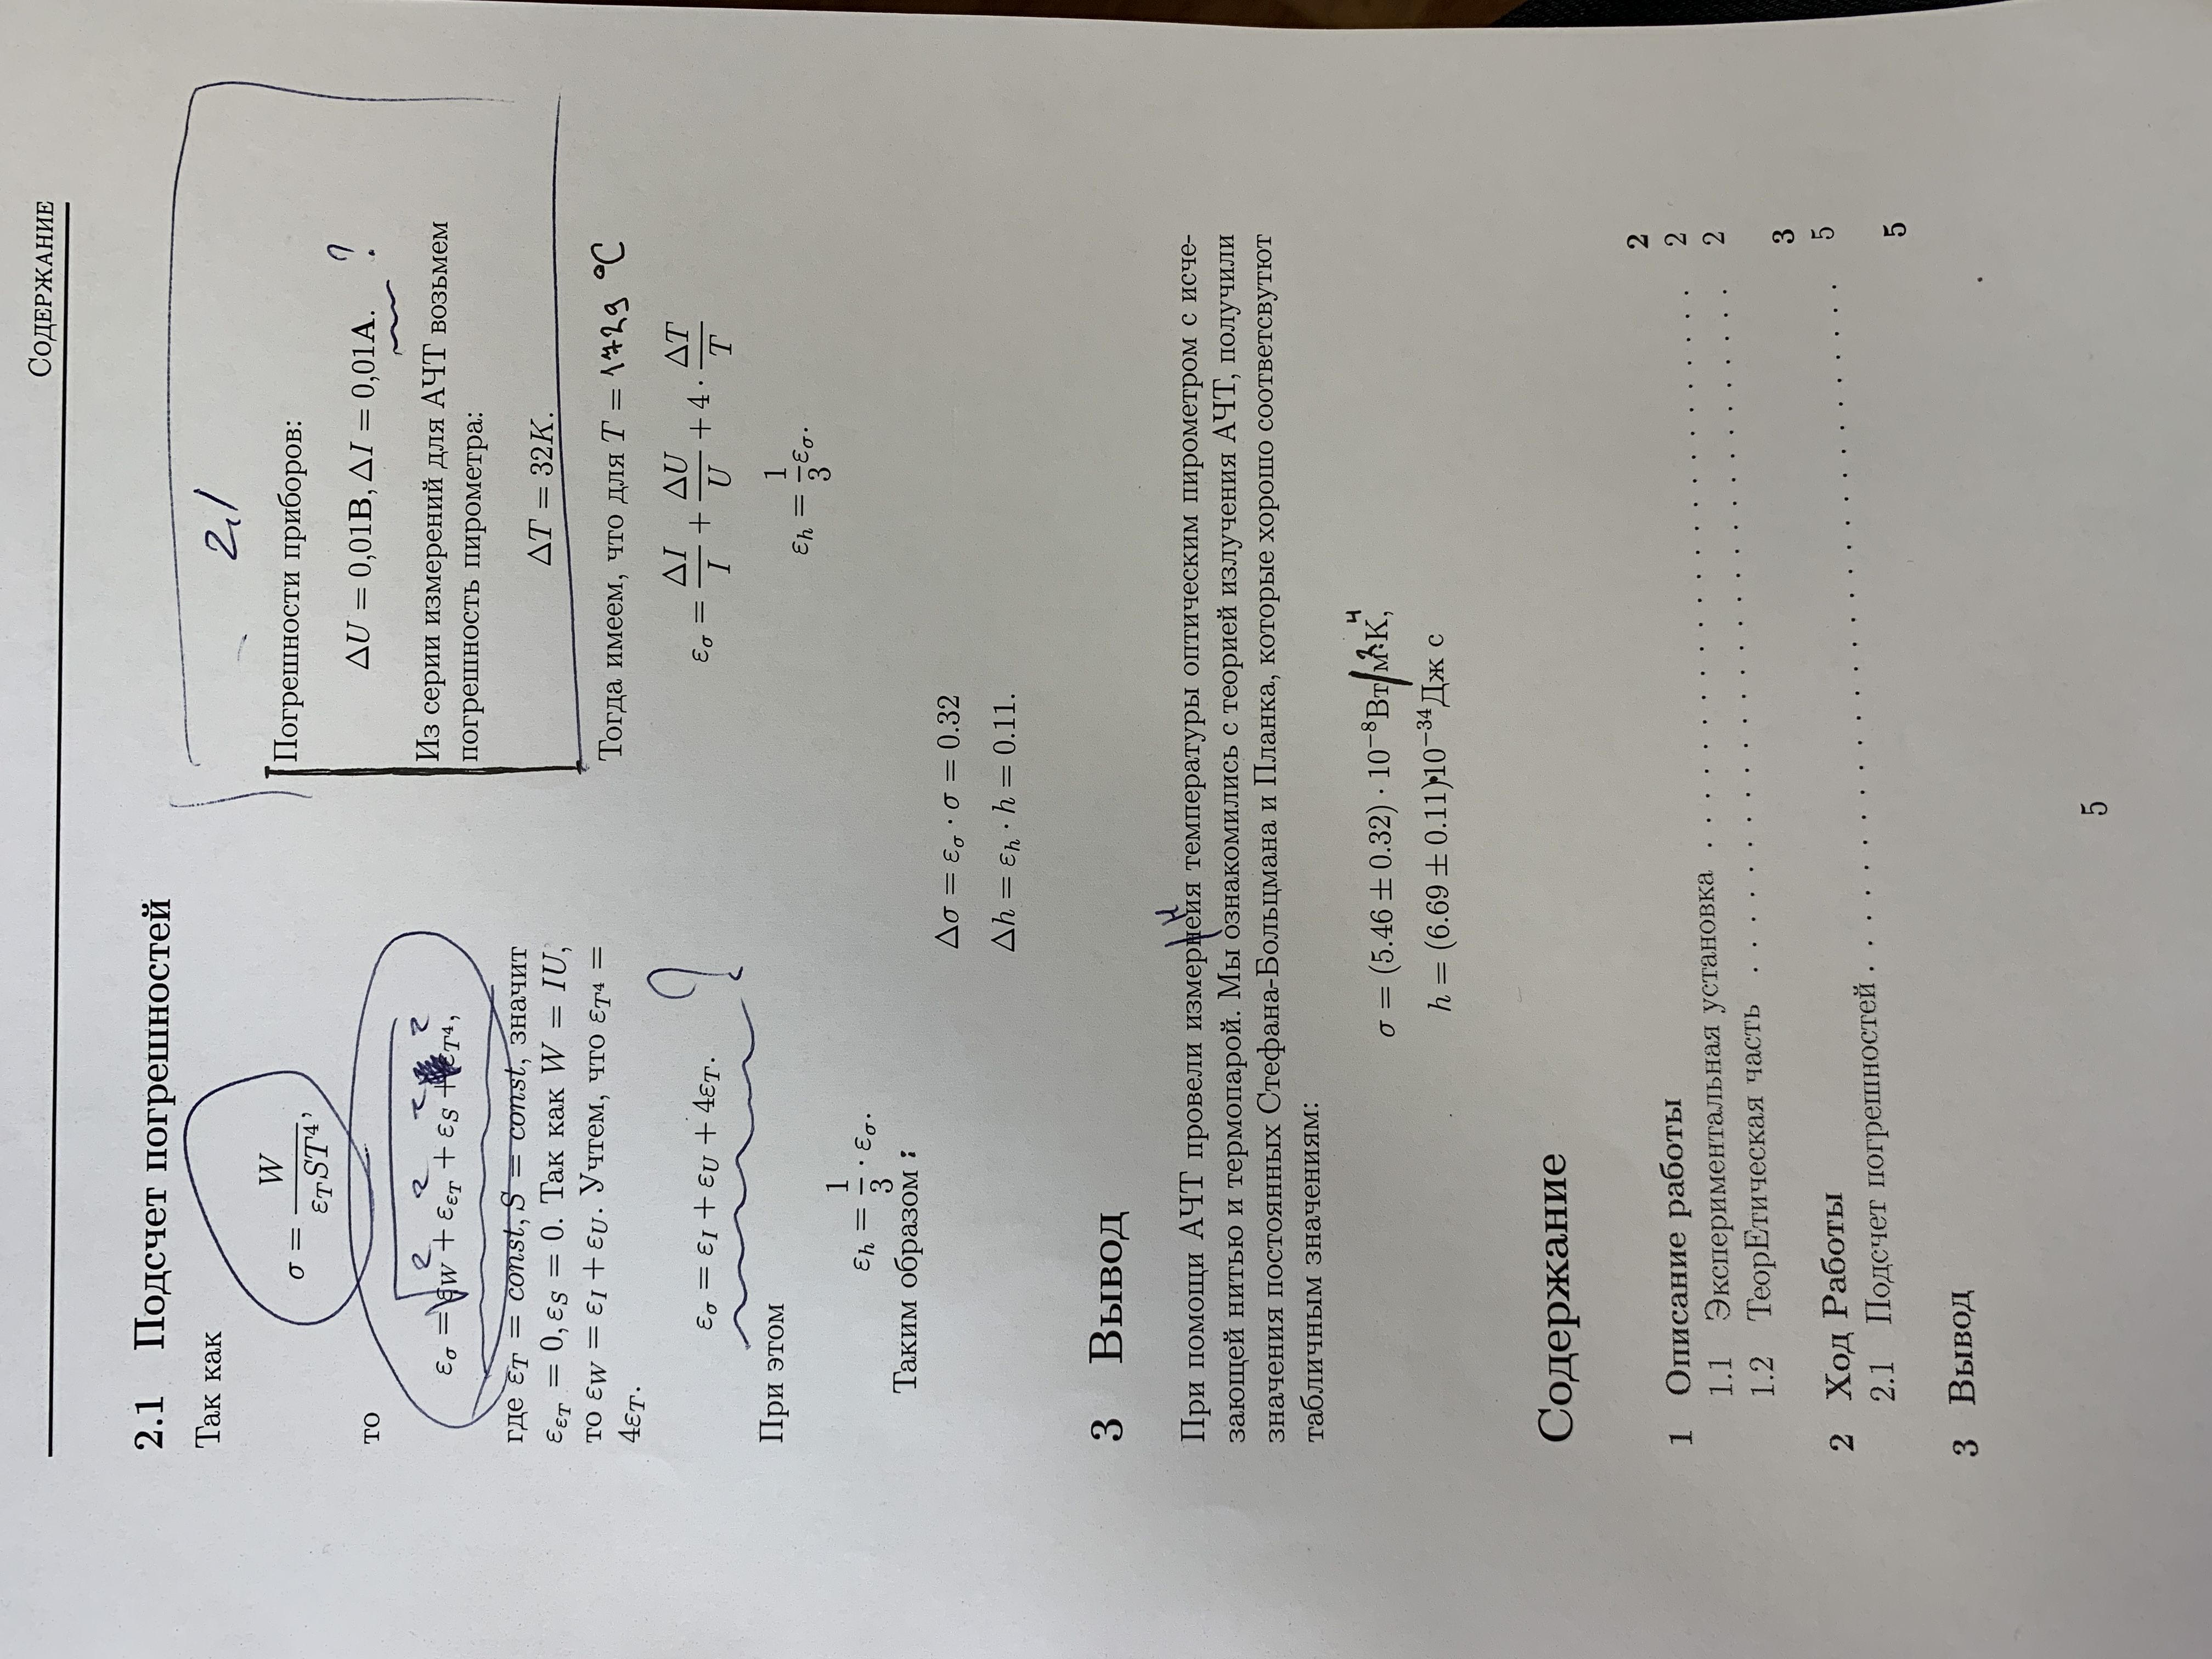
\includegraphics[width=1\textwidth,  angle = 270]{Materials/graph/IMG_2483.JPG}
    \caption{Схема установки}
\end{figure}

\end{document}